% This must be in the first 5 lines to tell arXiv to use pdfLaTeX.
\pdfoutput=1

\documentclass[11pt]{article}

% Remove the "review" option to generate the final version.
\usepackage[review]{ACL2023}

\usepackage{times}
\usepackage{latexsym}
\usepackage[T1]{fontenc}
\usepackage[utf8]{inputenc}
\usepackage{microtype}
\usepackage{inconsolata}
\usepackage{booktabs}
\usepackage{graphicx}

\title{Diagnose Before Simplifying: Operation-Aware Biomedical Text Simplification}

% TODO: fill in real author list / affiliations before submission
\author{
  Sruthilaya \and Rishabh \and Sophakotra \and Zihao \\
  Northeastern University \\
  \texttt{email@domain}
}

\begin{document}
\maketitle

\begin{abstract}
Biomedical text simplification is often treated as a single generation task
despite requiring different kinds of edits. We propose an operation-aware
framework that first predicts whether a sentence requires Substitution,
Explanation, or Generalization, then applies an operation-specific
simplification strategy. Complexity is characterized using complementary
lexical, syntactic, numerical, entity, and safety-critical signals, including
UMLS-based jargon detection. Under weak supervision, BioBERT achieves $0.465$
macro-F1 for operation prediction, outperforming TF-IDF ($0.424$) and
DistilBERT ($0.392$), while engineered UMLS features further improve the
TF-IDF baseline. Our complete pipeline combines deterministic CHV
substitution with constrained FLAN-T5 generation and protected-span
verification for the Substitution path. On the held-out PLABA test set, it
improves SARI over rule-based CHV ($21.72$ vs.\ $21.12$) while maintaining
perfect warning preservation, and preserves warnings and numerical content
better than direct FLAN-T5 generation. On a warning-stratified subset, it
also exceeds direct generation in SARI ($25.43$ vs.\ $24.73$). These results
support operation-aware routing as a controlled middle ground between
lexical substitution and unconstrained generation, and show that targeted,
safety-stratified evaluation can expose failures hidden by random sampling.
\end{abstract}

\section{Introduction}

Patient-facing biomedical text -- research abstracts, clinical notes, drug
labeling -- is frequently written at a reading and vocabulary level that assumes
clinical training the intended reader does not have. Low health literacy is linked
to worse health outcomes \citep{berkman2011health}, so making biomedical text
readable is a practical clinical concern, not only a linguistic one. Automated
simplification systems aim to close this gap, but most treat simplification as a
single, undifferentiated transformation applied uniformly across a text: a
sentence is fed into a model and a simpler sentence is returned, whether the
difficulty came from a single jargon term, a tangled clause structure, or a
critical dosage.

We argue this is the wrong framing. PLABA's own five-operation taxonomy
\citep{attal2023plaba} shows that ``simplify'' is not one transformation but
several distinct ones -- Substitution, Explanation, Generalization, Omission, and
Exemplification -- and prior work at the TSAR 2025 shared task confirms that no
submitted system, across 48 submissions from 20 teams, classifies which operation
a span needs before generating output \citep{alvamanchego2025tsarfindings}. We take
a diagnostic approach instead: classify first, then simplify. In this paper, we
operate at the \emph{sentence} level, not the sub-sentence span level the general
problem is sometimes framed at in prior work -- classifying one operation per
source sentence, rather than identifying and classifying multiple spans within a
single sentence, is the scope of our pseudo-labeling and classifier
(Section~\ref{sec:classifier-results}). Before any text is rewritten, we identify
what type of complexity a sentence carries, and only then apply the operation
suited to it. A jargon term can be replaced from a controlled vocabulary with no
free-form generation involved, avoiding generative hallucination at this step.
An unfamiliar concept can be
explained. An overly specific statement can be generalized. Routing each sentence
to the right operation lets us simplify aggressively where it is safe and stay
conservative where information must be preserved.

Our contributions are: (1) a multi-signal complexity detection framework
combining five complementary detectors (near-zero pairwise correlation among
the four with non-degenerate hit rates, strongest $\phi = 0.078$) with a
validated, production-grade UMLS jargon matcher that detects at least one
jargon candidate in every training abstract; (2) an operation classifier
progression
(TF-IDF $\rightarrow$ DistilBERT $\rightarrow$ BioBERT) suggesting biomedical-domain
pretraining is valuable for operation prediction, plus a controlled ablation showing
which of our detected features genuinely improve classification versus which are
better reserved for safety constraints at generation time; (3) an end-to-end evaluation of an operation-aware biomedical simplification pipeline against
uniform baselines, showing it improves readability over safe-but-limited
rule-based substitution while retaining that baseline's safety profile; (4) a
mechanism, currently implemented for our Substitution-routed generation path,
for using complexity detectors as \emph{generation-time guardrails}, not only
classifier inputs, verified post-hoc rather than merely requested of the
generator (Section~\ref{sec:chv-polish} discusses why this verification does
not yet extend to our Explanation/Generalization generation path); and (5) a
methodological finding that safety evaluation for simplification systems
requires warning-stratified sampling, since random sampling is statistically
underpowered to detect rare but safety-critical failures.

PLABA annotations show that simplification involves distinct operations:
Substitution ($64.7\%$), Explanation ($19.3\%$), Generalization ($6.3\%$),
with the remainder split between Omission and Exemplification
\citep{ondov2025lessons}. These operations are not interchangeable: lexical
lookup cannot produce explanations, while unrestricted generation can modify
information that should remain fixed. This asymmetry is especially important
in biomedical text. For example, simplifying \emph{``Do not exceed 2.5\,mg
daily''} to \emph{``Take the medicine daily''} improves surface readability
while deleting both a warning and an exact dosage. We therefore evaluate
readability jointly with warning and numerical preservation
(Section~\ref{sec:safety-eval}).

\section{Main Idea}
\label{sec:main-idea}

Figure-free summary of the architecture: a source sentence is first passed
through five complexity detectors (Section~\ref{sec:complexity-detection}) for
corpus-level diagnosis and safety-constraint extraction, and separately through
an operation classifier that predicts one of Substitution, Explanation, or
Generalization (Section~\ref{sec:classifier-results}).

The predicted operation determines the generation strategy: Substitution
routes to a Consumer Health Vocabulary (CHV) lookup, a deterministic,
auditable dictionary substitution with substantially lower hallucination risk
than free-form generation; Explanation and Generalization route to a
constrained large language model (FLAN-T5) prompted with an operation-specific
instruction, rather than a single generic ``simplify this'' prompt. Which
detector outputs feed the classifier as features, and how reliable our
pseudo-labels are, are both empirical questions we address with results
rather than assumptions, in Section~\ref{sec:classifier-results}.

\subsection{Complexity Detection Framework}
\label{sec:complexity-detection}

Before a biomedical sentence can be simplified, the system must first determine
\emph{what kind} of complexity it exhibits. We argue that biomedical text
complexity is not a single dimension but a composite of at least five distinct
signals, each requiring a different detection paradigm:

\begin{itemize}
    \item \textbf{Numerical expressions} (dosages, risk ratios, $p$-values,
    confidence intervals), detected via regular expressions. These patterns are
    finite and rule-governed, so no learned model is needed to achieve full
    recall on known formats.
    \item \textbf{Safety-critical warning language} (contraindications, adverse
    effects, risk alerts), detected via a hand-built lexicon, negation-aware (a
    sentence stating a warning does \emph{not} apply is not flagged). Because
    these phrases are clinically standardized, a lexicon provides an auditable,
    deterministic warning signal without requiring generative inference.
    \item \textbf{Named biomedical entities} (diseases, chemicals), detected via
    a supervised NER model (SciSpaCy, BC5CDR-trained; \citealp{neumann2019scispacy}).
    General-domain NER models miss domain-specific entities such as
    \emph{nephrotoxicity}; biomedical pretraining is not optional for this
    signal.
    \item \textbf{Structural complexity}, detected via dependency parse depth
    rather than raw sentence length. Length alone unfairly penalizes
    long-but-simple sentences (e.g., coordinated lists of facts), whereas parse
    depth captures genuine syntactic nesting that a vocabulary-only view misses
    entirely.
    \item \textbf{Medical jargon}, detected via UMLS concept matching
    (Section~\ref{sec:quickumls}). A term is treated as jargon if it exists in
    UMLS as a formal concept but is not part of common English vocabulary.
\end{itemize}

No single paradigm captures all five signals: regular expressions catch numbers
but miss entities; a lexicon catches warnings but misses syntactic structure; NER
catches entities but misses jargon that is not a named entity in the BC5CDR sense
(e.g., procedure names, qualifiers). We treat this as the central architectural
argument motivating a multi-detector design rather than a single end-to-end
classifier -- an argument reinforced empirically in
Section~\ref{sec:complexity-results}, where pairwise correlation among the
detectors is near zero wherever it is statistically defined.

\subsection{QuickUMLS Integration}
\label{sec:quickumls}

Our jargon detector is built on the Unified Medical Language System (UMLS), a
meta-thesaurus unifying over 200 source vocabularies (SNOMED CT, MeSH, RxNorm,
and others) into a single concept space of several million entries. We use
QuickUMLS \citep{Soldaini2016}, which maps free text to UMLS concept identifiers
via approximate string matching, to perform this lookup at the sentence level.

\paragraph{Definition of jargon.} A term is flagged as jargon if it resolves to a
UMLS concept \emph{and} is not part of common English vocabulary, operationalized
via three filters layered on top of raw QuickUMLS output:

\begin{enumerate}
    \item \textbf{Semantic type restriction.} UMLS concepts are tagged with one
    or more of 127+ semantic types. We restrict matches to eight clinically
    relevant types (e.g., \textit{Disease or Syndrome}, \textit{Pharmacologic
    Substance}, \textit{Therapeutic or Preventive Procedure}), excluding generic
    administrative or qualifier concepts that are technically present in UMLS
    but are already plain English (e.g., \textit{primary}, \textit{performed}).
    \item \textbf{Similarity threshold.} We require a QuickUMLS similarity score
    of at least 0.85, filtering out loose or uncertain string matches.
    \item \textbf{Lexical frequency filter.} Semantic-type restriction alone is
    insufficient: some common English words coincidentally match real,
    clinically-relevant UMLS concepts. For example, \emph{control} matches a
    genuine pharmacologic-substance concept at similarity 1.0 -- the same
    semantic type needed to correctly catch real drug names such as
    \emph{sorafenib}. We therefore apply a word-frequency filter using Zipf
    frequency scores \citep{wordfreq}, requiring single-word matches to fall
    below a threshold of 3.8 to be treated as jargon. This threshold was
    validated against a held-out set of 16 known common and jargon terms,
    cleanly separating common words (\emph{control}: 5.40, \emph{determine}:
    4.63, \emph{disease}: 4.90) from genuine jargon (\emph{carcinoma}: 3.15,
    \emph{hyperglycemia}: 2.31, \emph{sorafenib}: 1.43). A preliminary attempt
    using a broad English wordlist (NLTK's \texttt{words} corpus) was rejected:
    it classified genuine jargon such as \emph{hyperglycemia} as ordinary
    English, since raw dictionary membership does not capture actual usage
    frequency.
\end{enumerate}

Additionally, since QuickUMLS returns every candidate concept considered for a
matched span rather than a single best match, we deduplicate by retaining only
the highest-similarity candidate per span.

\section{Details, Evaluation, and Results}
\label{sec:results}

\subsection{Safety Evaluation Methodology}
\label{sec:safety-eval}

We measure whether a simplification system preserves safety-critical content
(contraindications, adverse effect warnings) using a warning-preservation metric
with paraphrase matching, rather than surface $n$-gram overlap metrics such as
ROUGE. ROUGE cannot distinguish between a system that preserves a warning and one
that silently drops it, provided the rest of the sentence is scored favorably;
our metric targets exactly this failure mode. We similarly measure numerical
preservation (exact dosage and statistic survival) and, where a NER environment is
available, entity preservation.

A central methodological finding from our evaluation is that \textbf{random
sampling is statistically underpowered to detect rare safety failures}.
Warning-bearing sentences occur at an overall rate of approximately $5.7\%$
across the combined train, validation, and test sentence-level pairs before
source-level deduplication ($519/9{,}085$). The corresponding held-out split
rates differ slightly: $6.4\%$ on validation ($73/1{,}141$) and $4.9\%$ on
test ($49/1{,}000$). Separately, $31.3\%$ of training abstracts contain at
least one warning-bearing sentence; this is an abstract-level statistic and
therefore not directly comparable to the sentence-level rates above. A random
sample of 50 sentences showed all baseline
systems achieving perfect warning preservation, a misleadingly optimistic result.
Only a \emph{stratified} stress test -- restricted to warning-bearing sentences
specifically -- revealed that unguided LLM-based simplification is the only
baseline that drops safety-critical content under evaluation.

The warning-stratified samples are small ($n=30$--$73$), so we interpret
preservation differences cautiously; for example, $0.980$ on the
49-sentence test subset may represent approximately one failure. Our claim
is therefore methodological rather than a broad claim that generative
systems are unsafe: stratified evaluation exposed a failure that a random
50-sentence evaluation missed entirely. This motivates targeted stress
testing alongside aggregate metrics for safety-critical NLP.

\subsection{Complexity Coverage Results}
\label{sec:complexity-results}

Table~\ref{tab:complexity-coverage} reports detector flag rates across our
verified training split ($n=530$ abstracts\footnote{We note a discrepancy
between this figure and an earlier internal estimate of $n=635$; the current
figure was independently re-derived via two methods (direct exclusion of
validation/test PMIDs from the source data, and the shipped train/validation/test
split file) which agree with each other. \texttt{train.csv} contains 635 rows but
531 unique PMIDs (530 after excluding one row with a blank PMID) -- 104 PMIDs have
two adaptation-version rows each. We report the verified, deduplicated number
here.}), comparing our real UMLS-based jargon detector against a
morphological (suffix-pattern) fallback baseline.

\begin{table}[t]
\centering
\small
\begin{tabular}{lrr}
\toprule
\textbf{Detector} & \textbf{Morph.} & \textbf{UMLS} \\
\midrule
NER              & --    & 98.7\% \\
Warning cues      & --    & 31.3\% \\
Syntactic depth   & 94.0\% & 94.0\% \\
Numerical exprs.  & --    & 60.4\% \\
Jargon (UMLS)     & 86.8\% & \textbf{100.0\%} \\
\midrule
3+ detectors firing & 90.8\% & 98.1\% \\
\bottomrule
\end{tabular}
\caption{Percentage of abstracts ($n=530$) in which each detector fires at
least once -- an abstract-level hit-rate, not a per-mention recall figure.
``Morph.'' denotes a suffix/pattern heuristic fallback used when a full UMLS
installation is unavailable; ``UMLS'' denotes the full QuickUMLS pipeline
described in Section~\ref{sec:quickumls}.}
\label{tab:complexity-coverage}
\end{table}

UMLS detected at least one jargon candidate in 100.0\% of training abstracts,
compared with 86.8\% under the morphological fallback. We are careful about what
this figure does and does not claim: it is an abstract-level hit-rate --
whether \emph{any} jargon was flagged per abstract -- not a per-mention recall
measurement, and it does not establish that every individual jargon expression
in the dataset was detected. Read this way, it is still a meaningful, direct
demonstration of a coverage gap between rule-based jargon detection and true
terminology-base lookup: the morphological heuristic fails to flag any
jargon candidate in $13.2\%$ of abstracts where the UMLS pipeline still
fires. We validated this result in two stages: first
against a small set of targeted test sentences containing known jargon (e.g.,
\emph{hepatocellular carcinoma}, \emph{sorafenib}, \emph{nephrotoxicity}), and
second via manual review of a random sample of ten training abstracts, confirming
that flagged terms were genuine clinical terminology (e.g., \emph{implantable
cardioverter-defibrillator}, \emph{hyporeninemic hypoaldosteronism},
\emph{gabapentinoids}) rather than residual false positives.

Consistent with our preliminary findings, the majority of abstracts exhibit
multiple simultaneous complexity signals: 98.1\% of abstracts trigger three or
more of our five detectors under the full UMLS pipeline. Note that individual
detector hit-rates vary widely (Table~\ref{tab:complexity-coverage}): UMLS
jargon and NER fire on nearly every abstract ($100.0\%$ and $98.7\%$
respectively), while warning cues and numerical expressions fire on a
minority ($31.3\%$ and $60.4\%$). We computed pairwise phi-coefficient
correlation at the abstract level ($n=530$) to test complementarity directly,
and we flag an important limitation of this specific statistic: UMLS jargon
fires on $100.0\%$ of abstracts with zero variance at this level of
aggregation, so its phi coefficient with every other detector is
mathematically degenerate (undefined, computed here as $0$ by convention)
rather than a genuine measurement of independence -- a constant variable
cannot be correlated with anything. We therefore report phi coefficients
only among the four detectors with non-degenerate abstract-level variance
(NER, warning, syntactic, numerical); among these, correlation is close to
zero across the board (strongest: NER-warning, $\phi = 0.078$), indicating
that \emph{these four} detectors are complementary rather than redundant
with one another. We do not extend this specific correlational claim to
UMLS jargon, whose complementarity with the other detectors is established
instead by its high, near-universal hit rate combined with the other
detectors' comparatively low hit rates -- if UMLS jargon were redundant with,
e.g., warning cues, we would expect abstracts without a warning cue to
also lack a UMLS jargon match, which the co-occurrence counts
(Table~\ref{tab:complexity-coverage}) do not support. We do not claim any of
this demonstrates five is the optimal number of detectors, or that this
exact combination is uniquely necessary -- only that treating biomedical
complexity as one-dimensional, as a single-signal detector does, would
systematically miss information that at least one of these five detectors is
capturing.

\subsection{Operation Classification}
\label{sec:classifier-results}

Predicting the operation a sentence requires is the research centerpiece. We
classify at the sentence level -- one operation label per source sentence --
rather than identifying and labeling operations for sub-sentence spans; extending
to finer-grained span-level classification within a sentence is future work
(Section~\ref{sec:conclusion}). Crucially, the classifier sees only the
\emph{source} sentence: at inference time no target exists, so any feature
derived from the reference would be leakage.

\paragraph{Pseudo-labeling.} Because PLABA lacks public sentence-level operation
labels, we derive them by weak supervision from aligned source-target pairs,
sentence-aligning \texttt{data.json} and excluding all validation and test PMIDs
to prevent leakage. Each pair is labeled by a length-ratio rule with an
edit-distance tiebreak: a target at least $15\%$ longer is an Explanation, one at
least $15\%$ shorter is a Generalization, and a similar-length pair with
sufficient character-level change is a Substitution. This yields $6{,}307$ labeled
training pairs: $43.2\%$ Substitution, $34.4\%$ Explanation, $22.5\%$
Generalization.

This pseudo-label distribution diverges substantially from the real,
human-annotated distribution that \citet{ondov2025lessons} report for the same
three operations ($64.7\%$ Substitution, $19.3\%$ Explanation, $6.3\%$
Generalization) -- Generalization is roughly $3.6\times$ over-represented in our
pseudo-labels. We believe this reflects a structural limitation of the
length-ratio heuristic: a source sentence that loses a numerically dense
subordinate clause (arguably an Omission-type edit) also shrinks in length and can
be indistinguishable, under a pure length-ratio rule, from a genuinely generalized
statement. We report our classifier results below against this caveat rather than
treating the pseudo-labels as gold. Given this gap between our weak-supervision
signal and the true operation distribution, we frame the entire classifier
experiment accordingly: our results should be interpreted as a
\emph{proof-of-concept for operation routing under weak supervision}, not as
a claim to a state-of-the-art, gold-label operation classifier. This framing
is also consistent with the broader PLABA literature, where operation
identification and classification is repeatedly reported as the harder
sub-problem -- \citet{ondov2025lessons} report human inter-annotator
agreement of only $0.46$ F1 on this exact task, and prior baseline
classifiers in the $0.33$--$0.39$ macro-F1 range -- while generation
\emph{conditioned on} a known operation is comparatively well-studied and
easier. Read this way, a macro-F1 in the $0.42$--$0.47$ range is a
reasonable proof-of-concept result on a task the field's own human
annotators do not agree on much more reliably, not a shortfall against a
mature, well-defined classification target.

\paragraph{Classifier progression.} Table~\ref{tab:classifier-progression}
reports macro-F1 across three classifier backbones: a lexical baseline, a
general-domain contextual model, and a biomedical-domain contextual model.
TF-IDF with $(1,2)$-gram features and class-weighted logistic regression
establishes the lexical baseline. DistilBERT, a general-domain contextual
model, actually \emph{underperforms} the lexical baseline by $7.5\%$
relative. BioBERT, pretrained on biomedical text specifically, improves over
TF-IDF by $9.7\%$ relative, and this result reproduced independently within
$1\%$ absolute macro-F1 across three separate training runs (0.465, 0.461,
0.467), indicating the result is not an artifact of training randomness. We
read this pattern as evidence that biomedical-domain pretraining is valuable
for operation prediction, since BioBERT outperforms both the lexical
baseline and the evaluated general-domain contextual baseline; we stop short
of claiming this isolates domain adaptation as the sole cause, since
DistilBERT and BioBERT also differ in architecture (6 vs.\ 12 transformer
layers) and parameter count, confounded with pretraining domain in this
comparison.

\begin{table}[t]
\centering
\small
\begin{tabular}{lr}
\toprule
\textbf{Model} & \textbf{Macro-F1} \\
\midrule
TF-IDF + Logistic Regression & 0.424 \\
DistilBERT                   & 0.392 \\
BioBERT                      & \textbf{0.465} \\
\bottomrule
\end{tabular}
\caption{Operation classifier progression on the PLABA validation set
($n=1{,}431$ pseudo-labeled sentence pairs).}
\label{tab:classifier-progression}
\end{table}

BioBERT's confusion matrix reveals where difficulty concentrates across all
three training runs: Generalization is consistently its weakest class (F1
$0.365$--$0.423$, recall $29$--$32\%$ depending on the run), confused almost
equally with both Substitution and Explanation, whereas contextual
pretraining substantially improved Explanation recall over the TF-IDF
baseline ($35\% \rightarrow 55\%$ in the run used for the deployed
classifier). We attribute Generalization's persistent difficulty at least
partly to the pseudo-label noise described above, rather than purely to
architectural capacity, since label noise likely limits achievable
classifier performance.

\paragraph{Feature integration (corrected ablation).}
\label{sec:feature-ablation}
We tested whether adding our detected UMLS jargon, warning, and numerical
features to the TF-IDF classifier improves operation prediction. An initial
version of this experiment compared a feature-augmented model built with a
smaller TF-IDF vocabulary ($5{,}000$ features) against a baseline built with a
larger one ($50{,}000$ features), confounding the effect of adding features with
the effect of shrinking the vocabulary -- the reported result (a small
\emph{decrease} in macro-F1) was consequently uninterpretable. Re-run with
matched vocabulary size, the corrected result reverses: adding UMLS and
numerical features improves macro-F1 by $0.021$--$0.025$ absolute over
TF-IDF alone (Table~\ref{tab:feature-ablation}).

\begin{table}[t]
\centering
\small
\begin{tabular}{lr}
\toprule
\textbf{Model} & \textbf{Macro-F1} \\
\midrule
TF-IDF only                        & 0.424 \\
\ + UMLS only (3 feat.)             & 0.443 \\
\ + UMLS + Numerical (6 feat.)      & 0.445 \\
\ + UMLS + Warning + Num.\ (8 feat.) & 0.449 \\
\bottomrule
\end{tabular}
\caption{Feature-integration ablation, TF-IDF backbone, corrected for the
vocabulary-size confound.}
\label{tab:feature-ablation}
\end{table}

A per-feature-group ablation isolates which features are responsible: UMLS
jargon features alone account for $76\%$ of the total gain, confirmed by
inspecting the trained model's coefficients directly (mean $|$coefficient$|$
for the engineered features is $0.124$, versus $0.084$ for an average TF-IDF
token -- these features are being weighted meaningfully, not diluted by 50,000
lexical dimensions). Warning features contribute approximately zero in
isolation ($+0.0008$ macro-F1), which we do \emph{not} treat as a shortcoming:
warning language indicates whether output is \emph{safe}, not \emph{which
operation} a sentence requires, and its value lies in the generation-time
constraint described in Section~\ref{sec:chv-polish}, not in routing accuracy.
Numerical features are the subtle case: alone, they measurably \emph{hurt}
Generalization F1 ($0.410 \rightarrow 0.387$) despite raw numerical-expression
presence correlating $2.2\times$ higher in true Generalization sentences than
Explanation sentences in the underlying data -- we interpret this as the
numerical signal being entangled with the same pseudo-label noise affecting
Generalization generally, rather than the feature itself being uninformative.

\subsection{Operation-Aware Generation and CHV-then-Polish}
\label{sec:chv-polish}

The predicted operation determines the generation strategy: Substitution routes
to CHV lookup, a deterministic dictionary substitution; Explanation and
Generalization route to FLAN-T5 with an operation-specific constrained prompt
in place of a single generic instruction.

An initial version of the full pipeline, evaluated against the three baselines
on the complete validation set, scored a SARI of only $18.76$ -- barely above
Rule-based CHV's $19.06$ -- because $43\%$ of sentences (Substitution-routed)
received only a flat dictionary word-swap with no fluency improvement. We
addressed this with a second generation step for Substitution-routed sentences:
after CHV substitution, an optional FLAN-T5 fluency-polish pass rewrites the
sentence for naturalness, constrained by an explicit list of protected spans
drawn directly from our complexity detectors -- the numerical expressions and
the CHV replacement terms just inserted -- injected into the prompt as spans
that must not change, and \emph{verified post-hoc}: if any protected span is
absent from the polished output, the pipeline discards it and falls back to the
deterministic CHV-only result rather than trusting the instruction was
followed. This is the sense in which complexity detection functions as a
generation-time guardrail (Section~\ref{sec:main-idea}), not only a classifier
feature.

An intermediate version of this mechanism, protecting only numerical spans and
CHV replacement terms, raised SARI to $20.09$ but measurably reduced warning
preservation from $1.000$ to $0.986$: a Substitution-routed sentence that
happened to also contain a warning phrase had that phrase left unprotected, and
the polish pass occasionally reworded it. Adding the warning detector's matched
phrases to the same protected-span list fully recovered warning preservation to
$1.000$ \emph{and} pushed SARI higher still, to $20.22$ -- a genuine improvement
on both axes from the same fix, not a trade-off, and itself a small
demonstration of the paper's broader argument: the failure mode only became
visible, and only became fixable, because we evaluated on both a readability
metric and a safety metric simultaneously.

\paragraph{Scope of the protected-span guardrail.} The protected-span
verification currently applies only to Substitution-routed CHV-then-polish
outputs; Explanation and Generalization use constrained prompts without
equivalent post-hoc verification. On the validation warning subset, only
$29/73$ sentences were routed through the protected path, yet the full
system retained $1.000$ warning preservation. We treat this as an empirical
observation rather than a guarantee; extending verification to all
generative routes is future work (Section~\ref{sec:conclusion}).

\subsection{Full-System Evaluation}
\label{sec:full-eval}

We report the complete comparison on the held-out PLABA \emph{test} set
($n=1{,}000$ sentences overall; $n=49$ warning-bearing sentences in the
stratified stress test), with the full pipeline configuration -- classifier
hyperparameters, CHV dictionary, and generation prompts -- frozen exactly as
selected during validation, so no test-set information influenced any design
decision. The classifier checkpoint deployed for this evaluation is one of
the three independent BioBERT training runs reported in
Section~\ref{sec:classifier-results} (macro-F1 $0.467$), re-trained under
identical settings after an unrelated infrastructure incident rather than
reused verbatim from the validation-time run; we note this explicitly rather
than implying a single frozen weight file, and its macro-F1's consistency
with the other two runs is itself evidence the specific training instance
does not materially affect the results reported below. All LLM-based
systems use matched decoding (beam search, 4 beams),
so differences in generation strategy do not confound the comparison. The
same evaluation was also run on the validation set during development
($n=1{,}141$ overall / $n=73$ stratified); we report test-set numbers as the
paper's headline result and note the validation-set pattern was consistent
throughout Section~\ref{sec:results}, not contradicted by the held-out run.

\begin{table}[t]
\centering
\small
\begin{tabular}{lrrr}
\toprule
\textbf{System} & \textbf{SARI} & \textbf{Warn.} & \textbf{Num.} \\
\midrule
No simplification    & 18.45 & 1.000 & 1.000 \\
Rule-based CHV        & 21.12 & 1.000 & 1.000 \\
Direct LLM (FLAN-T5)   & 25.49 & 0.980 & 0.925 \\
\textbf{Operation-aware} & \textbf{21.72} & \textbf{1.000} & 0.963 \\
\bottomrule
\end{tabular}
\caption{Full-system comparison, PLABA \emph{test} set, overall split
($n=1{,}000$). ``Warn.''/``Num.'' are warning/numerical preservation.}
\label{tab:full-results}
\end{table}

\begin{table}[t]
\centering
\small
\begin{tabular}{lrrr}
\toprule
\textbf{System} & \textbf{SARI} & \textbf{Warn.} & \textbf{Num.} \\
\midrule
No simplification    & 18.79 & 1.000 & 1.000 \\
Rule-based CHV        & 22.05 & 1.000 & 1.000 \\
Direct LLM (FLAN-T5)   & 24.73 & 0.980 & 0.818 \\
\textbf{Operation-aware} & \textbf{25.43} & \textbf{1.000} & 0.909 \\
\bottomrule
\end{tabular}
\caption{Full-system comparison, PLABA \emph{test} set, warning-stratified
stress test ($n=49$; small $n$ -- treat as indicative, see
Section~\ref{sec:safety-eval}).}
\label{tab:full-results-stratified}
\end{table}

On the full test split (Table~\ref{tab:full-results}), operation-aware
simplification improves over CHV in SARI ($21.72$ vs.\ $21.12$) and matches
its warning preservation ($1.000$), although numerical preservation falls
from $1.000$ to $0.963$. Relative to direct FLAN-T5, it trades SARI ($21.72$
vs.\ $25.49$) for stronger warning ($1.000$ vs.\ $0.980$) and numerical
preservation ($0.963$ vs.\ $0.925$). Thus, the overall result is a
controlled trade-off rather than universal dominance.

On warning-bearing sentences (Table~\ref{tab:full-results-stratified}), the
operation-aware system exceeds direct FLAN-T5 across all three measured
dimensions: SARI $25.43$ vs.\ $24.73$, warning preservation $1.000$ vs.\
$0.980$, and numerical preservation $0.909$ vs.\ $0.818$. Because $n=49$, we
treat the magnitude as indicative; importantly, the same qualitative pattern
appeared during validation. Together with BioBERT's stable performance
across three runs (Section~\ref{sec:classifier-results}), this suggests the
result is not driven by one favorable checkpoint or split.

Figure~\ref{fig:scatter-overall} and Figure~\ref{fig:scatter-stratified}
visualize both tables directly on the readability-safety plane: the overall
split shows a genuine trade-off frontier between our system and Direct LLM,
while the stratified split shows our system strictly dominating Direct LLM
on both axes simultaneously.

\begin{figure}[t]
\centering
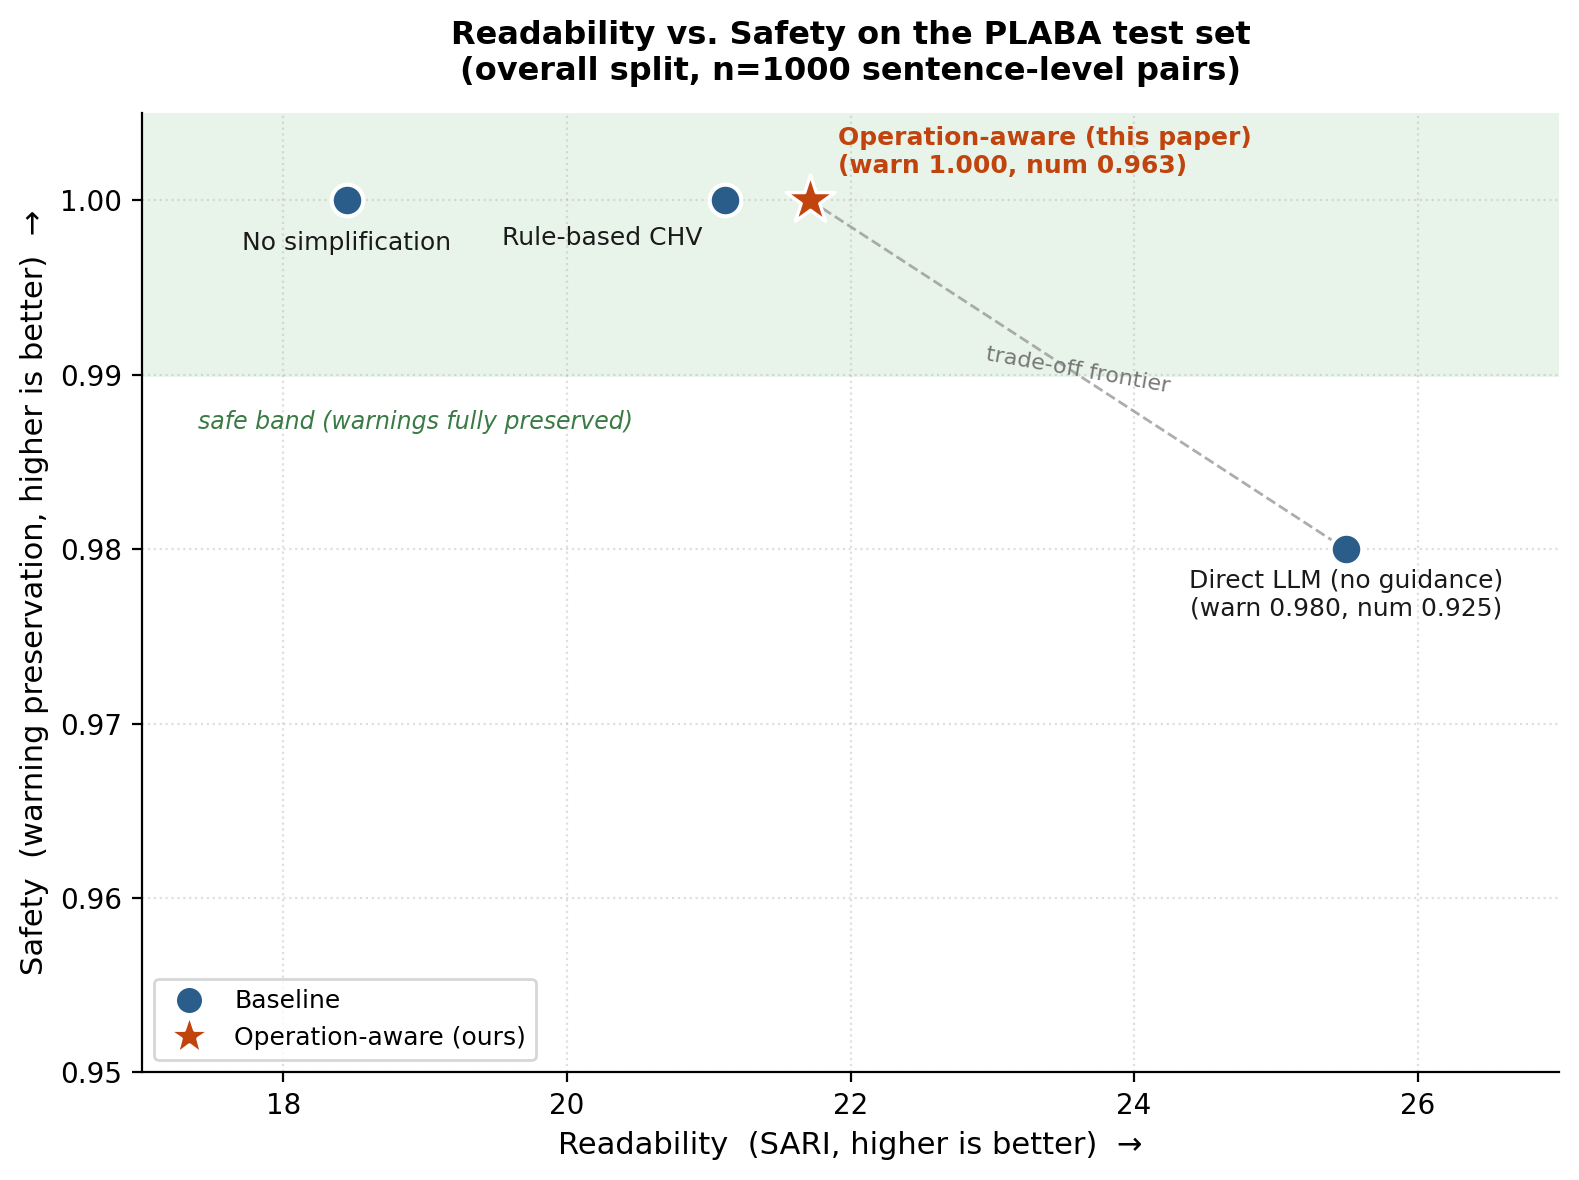
\includegraphics[width=\columnwidth]{../../results/readability_safety_scatter.png}
\caption{Readability (SARI) vs.\ safety (warning preservation) on the
overall test split ($n=1{,}000$). Our system and Rule-based CHV both sit in
the perfectly-safe band; our system reads better. Direct LLM reads better
still but exits the safe band.}
\label{fig:scatter-overall}
\end{figure}

\begin{figure}[t]
\centering
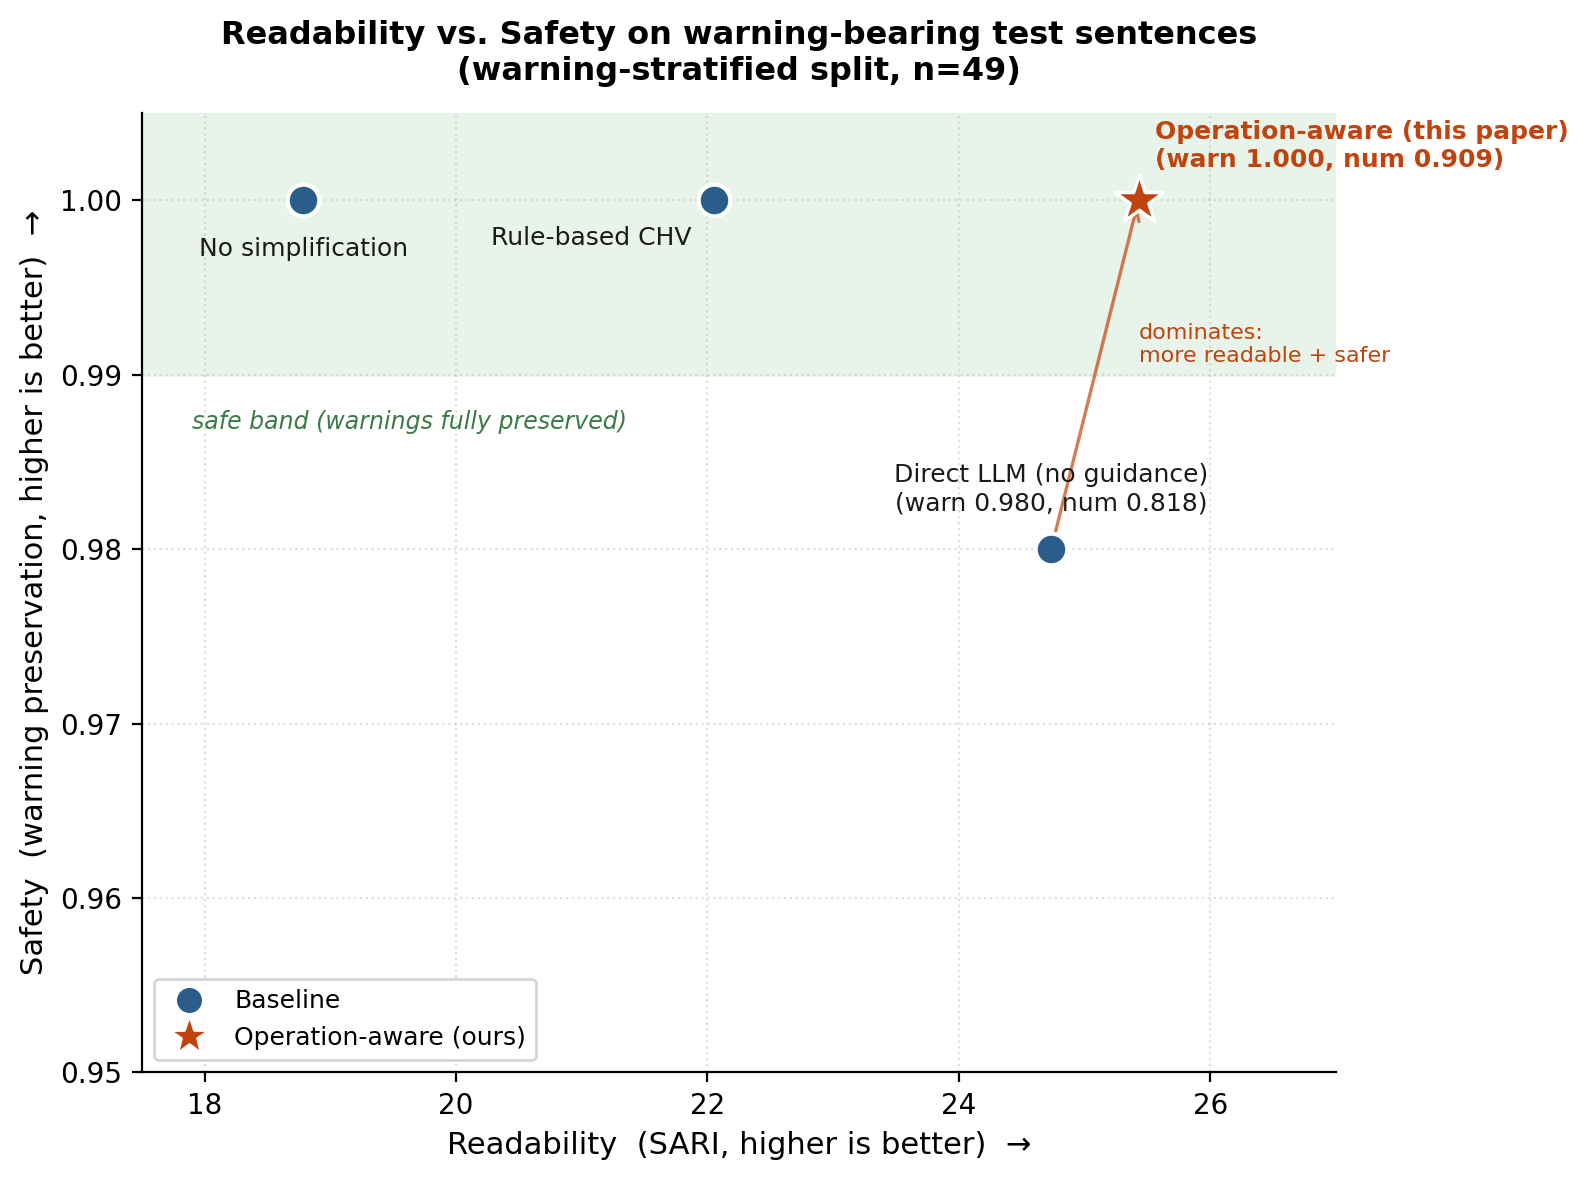
\includegraphics[width=\columnwidth]{../../results/readability_safety_scatter_stratified.png}
\caption{Same axes, restricted to the warning-stratified stress test
($n=49$). Here our system dominates Direct LLM outright -- higher SARI and
higher warning preservation simultaneously.}
\label{fig:scatter-stratified}
\end{figure}

\section{Related Work}

\paragraph{Datasets and prior PLABA systems.}
PLABA \citep{attal2023plaba} pairs biomedical abstracts with expert
plain-language rewrites at the sentence level, letting us pseudo-label
operations rather than treat simplification as opaque sequence-to-sequence
generation. \citet{knappich2023boschai}'s PLABA-2023-winning BoschAI
system finds that fine-tuned models copy the input and edit
little -- directly motivating our diagnostic framing, since a model that
barely edits also barely distinguishes a safe substitution from a
critical warning. \citet{li2024beemanc} investigate LLMs with
controllable attributes for the same track, including BART-based and
Lay-SciFive systems; we compare against a general-purpose LLM baseline
(FLAN-T5) and a rule-based baseline in this paper rather than against
these specific fine-tuned checkpoints, for reasons discussed in
Section~\ref{sec:conclusion}.

\paragraph{TSAR 2025 and the evaluation gap.}
The winning TSAR 2025 submission \citep{miyata2025ehimenlp} generates
candidates via 28 model-prompt combinations and reranks by semantic
similarity; their own ablation shows the gain comes from diversity and
selection, not from understanding \emph{what kind} of edit a span needs.
The shared task's own findings \citep{alvamanchego2025tsarfindings} show
that across 48 submissions from 20 teams, none classified complexity
type before generating output, and the official metrics (CEFR compliance,
MeaningBERT similarity) cannot detect a fluent output that quietly drops
a warning or dosage -- the organizers explicitly call for
expert-in-the-loop validation as future work. Our preservation metrics
answer this call by making safety a first-class, automatically measurable
criterion rather than deferring it to expert review.

\paragraph{Jargon detection and style robustness.}
\citet{papandreou2025jargon} show jargon detectors trained on MedReadMe
transfer poorly to PLABA ($33.71\%$ entity F1), since the datasets define
jargon under different annotation objectives -- supporting our decision to
build detectors natively on PLABA. Their jargon-aware LLM prompts also
introduce factual errors a lookup table structurally cannot produce,
motivating our CHV-based Substitution pathway over jargon-surfacing
prompts. \citet{rahman2025spqa} find that stylistic perturbations
significantly degrade LLM QA correctness and completeness even when
fluency stays stable, external evidence that surface-level metrics can
miss real content degradation -- the same gap our safety metrics target.

\paragraph{Prior operation-aware simplification.}
\citet{cripwell2022operation} propose controllable simplification via
operation classification as a predict-then-execute process, the same
structural intuition we extend to biomedical text at the sentence level.
\citet{devaraj2021medical} identify safety-critical information loss as a
recurring failure in paragraph-level medical simplification, directly
motivating our preservation metrics. \citet{xia2025jebs} introduce JEBS
on the same five-operation PLABA taxonomy, arguing that separating
identification, classification, and generation enables more targeted
evaluation -- the diagnose-before-simplify principle underlying our
pipeline.

\paragraph{Evaluation.}
SARI \citep{xu2016sari} rewards correct add/keep/delete operations against
multiple references; BERTScore \citep{zhang2020bertscore} adds contextual
semantic similarity. Neither captures whether a warning or dosage
survived, consistent with reports that SARI and FKGL correlate only
moderately with human judgment \citep{alvamanchego2021unsuitability} -- the
gap our preservation metrics are built to fill.

\section{Conclusion and Future Work}
\label{sec:conclusion}

We present a sentence-level operation-aware framework for biomedical text
simplification that routes Substitution, Explanation, and Generalization
through different simplification mechanisms rather than treating all inputs
as unrestricted generation. Under weak supervision, BioBERT provides the
strongest evaluated routing model, while UMLS-based features add signal
beyond TF-IDF lexical features. End-to-end evaluation shows that this
architecture moves beyond deterministic lexical substitution while improving
warning and numerical preservation relative to direct generation. On
warning-bearing test sentences, it also exceeds direct FLAN-T5 in SARI and
both preservation metrics, although the small sample warrants cautious
interpretation.

Our evaluation also highlights a methodological issue: aggregate or
random-sample evaluation can hide rare safety-critical failures.
Warning-stratified testing exposed a failure not observed under random
sampling, suggesting that safety-sensitive NLP evaluation should pair
overall quality metrics with targeted stress tests on high-risk subsets.

Future work should replace weak sentence-level pseudo-labels with gold or
span-level operation annotations, extend protected-span verification to
Explanation and Generalization, evaluate preservation with human judgments,
integrate engineered features with BioBERT directly, and compare against
specialized biomedical simplification models such as the BART-based and
Lay-SciFive systems of \citet{li2024beemanc}.

\section*{Limitations}
Our operation labels are weak sentence-level pseudo-labels and cannot
represent multiple operations within one sentence. UMLS jargon detection is
evaluated primarily through abstract-level hit rates and retains
phrase-level false positives. Protected-span verification currently covers
only the Substitution route, while Explanation and Generalization remain
prompt-constrained but unverified. Preservation metrics rely partly on
lexical matching and do not fully recognize valid paraphrases. The
warning-stratified test contains only 49 sentences, and evaluation is
limited to English PLABA data; broader datasets and human safety judgments
are needed.

\section*{Ethics Statement}
This work addresses a patient-safety concern: automated biomedical text
simplification that silently drops warnings or dosages could cause harm if
deployed without safeguards. None of the systems described here, including
our own, are validated for unsupervised clinical deployment; any real-world
use should retain human oversight (e.g., pharmacist or clinician review)
before reaching patients. We used only publicly available, de-identified
research abstracts (PLABA), and all models used (BioBERT, DistilBERT,
FLAN-T5) are open-weight and run locally, so no data processed by this
pipeline is transmitted to a third-party API.

\bibliography{anthology,custom}
\bibliographystyle{acl_natbib}

\end{document}
